\chapter{The Tidyverse}\label{tidyverse}

There is no point in becoming fluent in Enochian if you do not then call forth a Dweller Beneath at the time of the new moon.
Similarly,
there is no point learning a language designed for data manipulation if you do not then bend data to your will.
This chapter therefore looks at how to do the things that R was summoned---er, designed---to do,
and more specifically at a set of libraries called the \gref{g:tidyverse}{tidyverse}
designed to make data analyses easier to write and read~\cite{Wick2017}.

\section{How do we read data?}

We begin with the file \texttt{results/infant\_hiv.csv},
which reports the percentage of infants born to HIV-positive women
who received an HIV test themselves within two months of their birth.
The original data comes from \href{https://data.unicef.org/resources/dataset/hiv-aids-statistical-tables/}{UNICEF},
and Chapter~\ref{package} will show how to get from the messy original to a tidy version that contains:

\begin{lstlisting}
country,year,estimate,hi,lo
AFG,2009,NA,NA,NA
AFG,2010,NA,NA,NA
...
AFG,2017,NA,NA,NA
AGO,2009,NA,NA,NA
AGO,2010,0.03,0.04,0.02
AGO,2011,0.05,0.07,0.04
AGO,2012,0.06,0.08,0.05
...
ZWE,2016,0.71,0.88,0.62
ZWE,2017,0.65,0.81,0.57
\end{lstlisting}

The complete file has many more rows in place of the ellipses;
it uses \texttt{NA} to show missing data,
and its columns are:

\begin{longtable}[]{@{}lll@{}}
Header & Datatype & Description\\
country & char & ISO3 country code of country reporting data\\
year & integer & year CE for which data reported\\
estimate & double/NA & estimated percentage of measurement\\
hi & double/NA & high end of range\\
lo & double/NA & low end of range\\
\end{longtable}

We can read this data in Python like this \cite{Chen2017}:

\begin{lstlisting}
import pandas as pd

infant_hiv = pd.read_csv('results/infant_hiv.csv')
print(infant_hiv)
\end{lstlisting}

\begin{lstlisting}
     country  year  estimate    hi    lo
0        AFG  2009       NaN   NaN   NaN
1        AFG  2010       NaN   NaN   NaN
2        AFG  2011       NaN   NaN   NaN
3        AFG  2012       NaN   NaN   NaN
4        AFG  2013       NaN   NaN   NaN
5        AFG  2014       NaN   NaN   NaN
6        AFG  2015       NaN   NaN   NaN
7        AFG  2016       NaN   NaN   NaN
8        AFG  2017       NaN   NaN   NaN
...
\end{lstlisting}

To read this data in R,
we will load the \texttt{tidyverse} collection of \gref{g:package}{packages}
and then call the \texttt{read\_csv} function.
Let's start with the library:

\begin{lstlisting}
library(tidyverse)
\end{lstlisting}

\begin{lstlisting}
Error in library(tidyverse) : there is no package called
  'tidyverse'
\end{lstlisting}

\noindent
Ah.
We must install the tidyverse packages,
but only need to do so once per machine:

\begin{lstlisting}
install.packages("tidyverse")
\end{lstlisting}

\noindent
We then load the library into our R session:

\begin{lstlisting}
library(tidyverse)
\end{lstlisting}

\noindent
Note that we give \texttt{install.packages} a string \texttt{"tidyverse"},
but use the unquoted name \texttt{tidyverse} when we call \texttt{library}.

\begin{quote}
\textbf{What Do We Have Here?}

We can use \texttt{sessionInfo} to display what packages we have loaded,
along with the version of R we're using and some other useful information.
If you ever file a bug report for R,
please include this listing to help people help you.

\begin{lstlisting}
sessionInfo()
\end{lstlisting}

\begin{lstlisting}
R version 3.6.0 (2019-04-26)
Platform: x86_64-apple-darwin15.6.0 (64-bit)
Running under: macOS High Sierra 10.13.6

Matrix products: default
BLAS:   /Library/Frameworks/R.framework/Versions/3.6/Resources/lib/libRblas.0.dylib
LAPACK: /Library/Frameworks/R.framework/Versions/3.6/Resources/lib/libRlapack.dylib

locale:
[1] en_CA.UTF-8/en_CA.UTF-8/en_CA.UTF-8/C/en_CA.UTF-8/en_CA.UTF-8

attached base packages:
[1] stats     graphics  grDevices utils     datasets  methods   base     

other attached packages:
 [1] kableExtra_1.1.0 here_0.1         glue_1.3.1       knitr_1.24      
 [5] rlang_0.4.0      reticulate_1.12  forcats_0.4.0    stringr_1.4.0   
 [9] dplyr_0.8.3      purrr_0.3.2      readr_1.3.1      tidyr_1.0.0     
[13] tibble_2.1.3     ggplot2_3.2.1    tidyverse_1.2.1 

loaded via a namespace (and not attached):
 [1] tidyselect_0.2.5  xfun_0.8          haven_2.1.1      
 [4] lattice_0.20-38   colorspace_1.4-1  vctrs_0.2.0      
 [7] generics_0.0.2    viridisLite_0.3.0 htmltools_0.3.6  
[10] yaml_2.2.0        pillar_1.4.2      withr_2.1.2      
[13] modelr_0.1.5      readxl_1.3.1      lifecycle_0.1.0
...
\end{lstlisting}
\end{quote}

Loading the tidyverse gives us eight packages to play with.
One of those,
\texttt{dplyr},
defines two functions that mask pre-existing functions with the same names,
which is why the output of \texttt{library(tidyverse)} includes these two lines:

\begin{lstlisting}
dplyr::filter() masks stats::filter()
dplyr::lag()    masks stats::lag()
\end{lstlisting}

\noindent
If we need the original \texttt{filter} and \texttt{lag} functions,
we can always call them using with their
\gref{g:fully-qualified-name}{fully-qualified names}
\texttt{stats::filter} and \texttt{stats::lag}.

Once the tidyverse loaded is loaded,
reading our file looks remarkably like reading a file:

\begin{lstlisting}
infant_hiv <- read_csv('results/infant_hiv.csv')
\end{lstlisting}

\begin{lstlisting}
Parsed with column specification:
cols(
  country = col_character(),
  year = col_double(),
  estimate = col_double(),
  hi = col_double(),
  lo = col_double()
)
\end{lstlisting}

\texttt{read\_csv} tells us more about what it has done than its Pandas counterpart.
In particular,
it guesses the data types of columns based on the first thousand values
and then tells us what types it has inferred\footnote{In a better universe than this one,
people would consistently use the second row of their CSV files to tell us columns' types and units,
but we must live in this one.}.
We can now look at what \texttt{read\_csv} has produced:

\begin{lstlisting}
infant_hiv
\end{lstlisting}

\begin{lstlisting}
# A tibble: 1,728 x 5
   country  year estimate    hi    lo
   <chr>   <dbl>    <dbl> <dbl> <dbl>
 1 AFG      2009       NA    NA    NA
 2 AFG      2010       NA    NA    NA
 3 AFG      2011       NA    NA    NA
 4 AFG      2012       NA    NA    NA
 5 AFG      2013       NA    NA    NA
 6 AFG      2014       NA    NA    NA
 7 AFG      2015       NA    NA    NA
 8 AFG      2016       NA    NA    NA
 9 AFG      2017       NA    NA    NA
10 AGO      2009       NA    NA    NA
# ... with 1,718 more rows
\end{lstlisting}

\noindent
This is a \gref{g:tibble}{tibble},
which is the tidyverse's enhanced version of the \gref{g:data-frame}{data frame}
that R uses to store tabular data.
A tibble organizes data into named columns,
each having one value for each row.
In statistical terms,
the columns are the values being observed
and the rows are the actual observations.

\section{How do we inspect data?}

We often want to have a quick look at the contents of a table in memory.
Pandas does this using methods
whose names are borrowed from the Unix shell's \texttt{head} and \texttt{tail} commands:

\begin{lstlisting}
print(infant_hiv.head())
\end{lstlisting}

\begin{lstlisting}
  country  year  estimate  hi  lo
0     AFG  2009       NaN NaN NaN
1     AFG  2010       NaN NaN NaN
2     AFG  2011       NaN NaN NaN
3     AFG  2012       NaN NaN NaN
4     AFG  2013       NaN NaN NaN
\end{lstlisting}

\begin{lstlisting}
print(infant_hiv.tail())
\end{lstlisting}

\begin{lstlisting}
     country  year  estimate    hi    lo
1723     ZWE  2013      0.57  0.70  0.49
1724     ZWE  2014      0.54  0.67  0.47
1725     ZWE  2015      0.59  0.73  0.51
1726     ZWE  2016      0.71  0.88  0.62
1727     ZWE  2017      0.65  0.81  0.57
\end{lstlisting}

R has functions with similar names:

\begin{lstlisting}
head(infant_hiv)
\end{lstlisting}

\begin{lstlisting}
# A tibble: 6 x 5
  country  year estimate    hi    lo
  <chr>   <dbl>    <dbl> <dbl> <dbl>
1 AFG      2009       NA    NA    NA
2 AFG      2010       NA    NA    NA
3 AFG      2011       NA    NA    NA
4 AFG      2012       NA    NA    NA
5 AFG      2013       NA    NA    NA
6 AFG      2014       NA    NA    NA
\end{lstlisting}

\begin{lstlisting}
tail(infant_hiv)
\end{lstlisting}

\begin{lstlisting}
# A tibble: 6 x 5
  country  year estimate    hi    lo
  <chr>   <dbl>    <dbl> <dbl> <dbl>
1 ZWE      2012    0.38   0.47 0.33 
2 ZWE      2013    0.570  0.7  0.49 
3 ZWE      2014    0.54   0.67 0.47 
4 ZWE      2015    0.59   0.73 0.51 
5 ZWE      2016    0.71   0.88 0.62 
6 ZWE      2017    0.65   0.81 0.570
\end{lstlisting}

\noindent
Note that the row numbers printed by \texttt{head} and \texttt{tail}
are \gref{g:relative-row-number}{relative} to the output in R.
This is different from Python,
which displays the \gref{g:absolute-row-number}{absolute row number}
(i.e., the row's index within the original table).

What if we want some overall information about our data?
In Python we use a method called \texttt{.info}:

\begin{lstlisting}
print(infant_hiv.info())
\end{lstlisting}

\begin{lstlisting}
<class 'pandas.core.frame.DataFrame'>
RangeIndex: 1728 entries, 0 to 1727
Data columns (total 5 columns):
country     1728 non-null object
year        1728 non-null int64
estimate    728 non-null float64
hi          728 non-null float64
lo          728 non-null float64
dtypes: float64(3), int64(1), object(1)
memory usage: 67.6+ KB
None
\end{lstlisting}

\noindent
In R,
we can use a function called \texttt{summary},
which gives us quartiles and much more:

\begin{lstlisting}
summary(infant_hiv)
\end{lstlisting}

\begin{lstlisting}
   country               year         estimate           hi        
 Length:1728        Min.   :2009   Min.   :0.000   Min.   :0.0000  
 Class :character   1st Qu.:2011   1st Qu.:0.100   1st Qu.:0.1400  
 Mode  :character   Median :2013   Median :0.340   Median :0.4350  
                    Mean   :2013   Mean   :0.387   Mean   :0.4614  
                    3rd Qu.:2015   3rd Qu.:0.620   3rd Qu.:0.7625  
                    Max.   :2017   Max.   :0.950   Max.   :0.9500  
                                   NA's   :1000    NA's   :1000    
       lo        
 Min.   :0.0000  
 1st Qu.:0.0800  
 Median :0.2600  
 Mean   :0.3221  
 3rd Qu.:0.5100  
 Max.   :0.9500  
 NA's   :1000    
\end{lstlisting}

\noindent
Your output may or may not wrap
depending on how large a screen the older acolytes have allowed you.

\section{How do we index rows and columns?}

A Pandas \texttt{DataFrame} is a collection of \texttt{Series} objects,
each of which makes up a column in the overall table.
We can access these by name:

\begin{lstlisting}
print(infant_hiv['estimate'])
\end{lstlisting}

\begin{lstlisting}
0        NaN
1        NaN
2        NaN
3        NaN
4        NaN
5        NaN
6        NaN
7        NaN
8        NaN
9        NaN
10      0.03
11      0.05
12      0.06
...
\end{lstlisting}

\noindent
We would get exactly the same output in Python with \texttt{infant\_hiv.estimate},
i.e.,
by using the column name as an attribute rather than as an array subscript.
We can similarly use both strings and attributes in R:

\begin{lstlisting}
infant_hiv['estimate']
\end{lstlisting}

\begin{lstlisting}
# A tibble: 1,728 x 1
   estimate
      <dbl>
 1       NA
 2       NA
 3       NA
 4       NA
 5       NA
 6       NA
 7       NA
 8       NA
 9       NA
10       NA
# ... with 1,718 more rows
\end{lstlisting}

\begin{lstlisting}
infant_hiv$estimate
\end{lstlisting}

\begin{lstlisting}
   [1]   NA   NA   NA   NA   NA   NA   NA   NA   NA   NA 0.03 0.05
  [13] 0.06 0.15 0.10 0.06 0.01 0.01   NA   NA   NA   NA   NA   NA
  [25]   NA   NA   NA   NA   NA   NA   NA   NA   NA   NA   NA   NA
  [37]   NA   NA   NA   NA   NA   NA   NA   NA   NA   NA   NA 0.13
  [49] 0.12 0.12 0.52 0.53 0.67 0.66   NA   NA   NA   NA   NA   NA
  [61]   NA   NA   NA   NA   NA   NA   NA   NA   NA   NA   NA   NA
  [73]   NA   NA   NA   NA   NA   NA   NA   NA   NA   NA   NA   NA
  [85]   NA   NA   NA   NA   NA   NA 0.26 0.24 0.38 0.55 0.61 0.74
  [97] 0.83 0.75 0.74   NA 0.10 0.10 0.11 0.18 0.12 0.02 0.12 0.20
 [109]   NA   NA   NA   NA   NA   NA   NA   NA   NA   NA   NA 0.10
...
\end{lstlisting}

\noindent
As before,
the boxed number on the left is the index of the first item in that row.

What if we want a single value?
Remembering to count from zero for Python and as humans do for R,
we have:

\begin{lstlisting}
print(infant_hiv.estimate[11])
\end{lstlisting}

\begin{lstlisting}
0.05
\end{lstlisting}

\begin{lstlisting}
infant_hiv$estimate[12]
\end{lstlisting}

\begin{lstlisting}
[1] 0.05
\end{lstlisting}

\noindent
Ah---everything in R is a vector,
so the index \texttt{[12]} actually gives us a vector containing one value
rather than a raw value.
This is why we have to be careful \emph{not} to ask for the length of a single value in Python:
\begin{lstlisting}
print(len(1234))
\end{lstlisting}

\begin{lstlisting}
TypeError: object of type 'int' has no len()
\end{lstlisting}

\noindent
but can ask for the length of pretty much anything in R:

\begin{lstlisting}
length(1234)
\end{lstlisting}

\begin{lstlisting}
[1] 1
\end{lstlisting}

\section{How do we select ranges?}

As we saw in Chapter~\ref{basics},
we can use \gref{g:range-expression}{range expressions} to select multiple values in both languages:

\begin{lstlisting}
print(infant_hiv.estimate[5:15])
\end{lstlisting}

\begin{lstlisting}
5      NaN
6      NaN
7      NaN
8      NaN
9      NaN
10    0.03
11    0.05
12    0.06
13    0.15
14    0.10
Name: estimate, dtype: float64
\end{lstlisting}

\begin{lstlisting}
infant_hiv$estimate[6:15]
\end{lstlisting}

\begin{lstlisting}
 [1]   NA   NA   NA   NA   NA 0.03 0.05 0.06 0.15 0.10
\end{lstlisting}

The lower bounds are different because of 0~vs.~1-based counting.
The upper bound is the same because it's \emph{inclusive} in R and \emph{exclusive} in Python.
Note that nothing in either language prevents us from selecting a range that spans several countries,
which is why selecting by row number is usually a sign of innocence, insouciance, or desperation.

We can select by column number as well.
Pandas requires the rather clumsy \texttt{object.iloc[rows, columns]}
with the usual shortcut \texttt{:} for ``entire range'':

\begin{lstlisting}
print(infant_hiv.iloc[:, 0])
\end{lstlisting}

\begin{lstlisting}
0       AFG
1       AFG
2       AFG
3       AFG
4       AFG
5       AFG
6       AFG
7       AFG
8       AFG
9       AGO
10      AGO
...
\end{lstlisting}

\noindent
Since this is a column,
we can subscript it further to get a single value:

\begin{lstlisting}
print(infant_hiv.iloc[:, 0][0])
\end{lstlisting}

\begin{lstlisting}
AFG
\end{lstlisting}

In R,
a single index is interpreted as a column index:

\begin{lstlisting}
infant_hiv[1]
\end{lstlisting}

\begin{lstlisting}
# A tibble: 1,728 x 1
   country
   <chr>  
 1 AFG    
 2 AFG    
 3 AFG    
 4 AFG    
 5 AFG    
 6 AFG    
 7 AFG    
 8 AFG    
 9 AFG    
10 AGO    
# ... with 1,718 more rows
\end{lstlisting}

However,
the result is not a vector:
it's a tibble with N rows and one column.
This means that adding another subscript does column-wise indexing on that tibble:

\begin{lstlisting}
infant_hiv[1][1]
\end{lstlisting}

\begin{lstlisting}
# A tibble: 1,728 x 1
   country
   <chr>  
 1 AFG    
 2 AFG    
 3 AFG    
 4 AFG    
 5 AFG    
 6 AFG    
 7 AFG    
 8 AFG    
 9 AFG    
10 AGO    
# ... with 1,718 more rows
\end{lstlisting}

\noindent
which gives us back exactly the same structure we started with.
How then are we to get the first mention of Afghanistan?
The answer is to use \gref{g:double-square-brackets}{double square brackets}
to strip away one level of structure:

\begin{lstlisting}
infant_hiv[[1]]
\end{lstlisting}

\begin{lstlisting}
   [1] "AFG" "AFG" "AFG" "AFG" "AFG" "AFG" "AFG" "AFG" "AFG" "AGO"
  [11] "AGO" "AGO" "AGO" "AGO" "AGO" "AGO" "AGO" "AGO" "AIA" "AIA"
  [21] "AIA" "AIA" "AIA" "AIA" "AIA" "AIA" "AIA" "ALB" "ALB" "ALB"
  [31] "ALB" "ALB" "ALB" "ALB" "ALB" "ALB" "ARE" "ARE" "ARE" "ARE"
  [41] "ARE" "ARE" "ARE" "ARE" "ARE" "ARG" "ARG" "ARG" "ARG" "ARG"
  [51] "ARG" "ARG" "ARG" "ARG" "ARM" "ARM" "ARM" "ARM" "ARM" "ARM"
  [61] "ARM" "ARM" "ARM" "ATG" "ATG" "ATG" "ATG" "ATG" "ATG" "ATG"
  [71] "ATG" "ATG" "AUS" "AUS" "AUS" "AUS" "AUS" "AUS" "AUS" "AUS"
  [81] "AUS" "AUT" "AUT" "AUT" "AUT" "AUT" "AUT" "AUT" "AUT" "AUT"
  [91] "AZE" "AZE" "AZE" "AZE" "AZE" "AZE" "AZE" "AZE" "AZE" "BDI"
 [101] "BDI" "BDI" "BDI" "BDI" "BDI" "BDI" "BDI" "BDI" "BEL" "BEL"
 [111] "BEL" "BEL" "BEL" "BEL" "BEL" "BEL" "BEL" "BEN" "BEN" "BEN"
 [121] "BEN" "BEN" "BEN" "BEN" "BEN" "BEN" "BFA" "BFA" "BFA" "BFA"
...
\end{lstlisting}

This is now a plain old vector,
so it can be indexed with \gref{g:single-square-brackets}{single square brackets}:

\begin{lstlisting}
infant_hiv[[1]][1]
\end{lstlisting}

\begin{lstlisting}
[1] "AFG"
\end{lstlisting}

But that too is a vector,
so naturally\footnote{For some large value of ``natural''{\ldots}}
it can be indexed as well:

\begin{lstlisting}
infant_hiv[[1]][1][1]
\end{lstlisting}

\begin{lstlisting}
[1] "AFG"
\end{lstlisting}

\noindent
Thus,
\texttt{data[1][[1]]} produces a tibble,
then selects the first column vector from it,
so it still gives us a vector.
\emph{This is not madness.}
It is just{\ldots}differently sane.

\begin{quote}
\textbf{Subsetting Data Frames}

When we are working with data frames (including tibbles),
subsetting with a single range selects columns rather than rows
because data frames are stored as lists of columns.
This means that \texttt{df[1:2]} selects two columns from \texttt{df}.
However, in \texttt{df[2:3, 1:2]},
the first range selects rows while the second selects columns.
\end{quote}

\section{How do we calculate basic statistics?}

What is the average of all the values in the \texttt{estimate} column?
We start by grabbing that column for convenience:

\begin{lstlisting}
estimates = infant_hiv.estimate
print(len(estimates))
\end{lstlisting}

\begin{lstlisting}
1728
\end{lstlisting}

\noindent
and then call a method to get the value we want:

\begin{lstlisting}
print(estimates.mean())
\end{lstlisting}

\begin{lstlisting}
0.3870192307692308
\end{lstlisting}

\noindent
This translates almost directly to R:

\begin{lstlisting}
estimates <- infant_hiv$estimate
length(estimates)
\end{lstlisting}

\begin{lstlisting}
[1] 1728
\end{lstlisting}

\begin{lstlisting}
mean(estimates)
\end{lstlisting}

\begin{lstlisting}
[1] NA
\end{lstlisting}

R's answer is both more correct and less useful:
more correct because we can't actually calculate the mean when some values are missing,
and less useful because we almost always want the mean of the values we have.
Let's fix this by telling \texttt{mean} to drop NAs:

\begin{lstlisting}
mean(estimates, na.rm = TRUE)
\end{lstlisting}

\begin{lstlisting}
[1] 0.3870192
\end{lstlisting}

\noindent
and then double back to get the statistically correct behavior in Pandas:

\begin{lstlisting}
print(estimates.mean(skipna=False))
\end{lstlisting}

\begin{lstlisting}
nan
\end{lstlisting}

Many functions in R use \texttt{na.rm}
to control whether \texttt{NA}s are removed or not\footnote{Remember,
  the \texttt{.} character is just another part of the name.}.
In general
R's default is to leave \texttt{NA}s in when doing \gref{g:aggregation}{aggregate} computations
while Python's is to get rid of missing values early and work with what's left,
which makes translating code from one language to the next much more interesting than it might otherwise be.
This is why we write:

\begin{lstlisting}
print("min", estimates.min())
print("max", estimates.max())
print("std", estimates.std())
\end{lstlisting}

\begin{lstlisting}
min 0.0
max 0.95
std 0.3034511074214113
\end{lstlisting}

\noindent
in Python but need the following in R:

\begin{lstlisting}
print(glue("min {min(estimates, na.rm = TRUE)}"))
print(glue("max {max(estimates, na.rm = TRUE)}"))
print(glue("sd {sd(estimates, na.rm = TRUE)}"))
\end{lstlisting}

\begin{lstlisting}
min 0
max 0.95
sd 0.303451107421411
\end{lstlisting}

\section{How do we filter data?}

To \gref{g:filter}{filter} data means to select records by value rather than index.
As discussed in Chapter~\ref{basics},
the simplest approach is to use a vector of logical values as an index.
In Python, we do this with:

\begin{lstlisting}
maximal = estimates[estimates >= 0.95]
print(len(maximal))
\end{lstlisting}

\begin{lstlisting}
52
\end{lstlisting}

\noindent
and in R:

\begin{lstlisting}
maximal <- estimates[estimates >= 0.95]
length(maximal)
\end{lstlisting}

\begin{lstlisting}
[1] 1052
\end{lstlisting}

The difference is unexpected.
Let's have a closer look at the result in Python:

\begin{lstlisting}
print(maximal)
\end{lstlisting}

\begin{lstlisting}
180     0.95
181     0.95
182     0.95
183     0.95
184     0.95
185     0.95
187     0.95
360     0.95
...
\end{lstlisting}

And in R:

\begin{lstlisting}
maximal
\end{lstlisting}

\begin{lstlisting}
   [1]   NA   NA   NA   NA   NA   NA   NA   NA   NA   NA   NA   NA
  [13]   NA   NA   NA   NA   NA   NA   NA   NA   NA   NA   NA   NA
  [25]   NA   NA   NA   NA   NA   NA   NA   NA   NA   NA   NA   NA
  [37]   NA   NA   NA   NA   NA   NA   NA   NA   NA   NA   NA   NA
  [49]   NA   NA   NA   NA   NA   NA   NA   NA   NA   NA   NA   NA
  [61]   NA   NA   NA   NA   NA   NA   NA   NA   NA   NA   NA   NA
  [73]   NA   NA   NA   NA   NA   NA   NA   NA   NA   NA   NA   NA
  [85]   NA   NA   NA   NA   NA   NA   NA   NA   NA   NA   NA   NA
  [97]   NA   NA   NA   NA   NA   NA   NA   NA   NA   NA   NA   NA
 [109]   NA   NA   NA   NA   NA   NA   NA   NA   NA   NA   NA   NA
 [121]   NA   NA   NA   NA 0.95 0.95 0.95 0.95 0.95 0.95 0.95   NA
 [133]   NA   NA   NA   NA   NA   NA   NA   NA   NA   NA   NA   NA
...
\end{lstlisting}

Once again,
R has kept missing values in order to highlight just how little we know.
More precisely,
wherever there was an \texttt{NA} in the original data
there is an \texttt{NA} in the logical vector
and hence an \texttt{NA} in the final vector.
If we want to discard these,
we can use \texttt{which} to get a vector of indices at which a vector contains \texttt{TRUE}.
This function does not return indices for \texttt{FALSE} or \texttt{NA}:

\begin{lstlisting}
which(estimates >= 0.95)
\end{lstlisting}

\begin{lstlisting}
 [1]  181  182  183  184  185  186  188  361  362  363  380  381  382
[14]  383  385  386  387  447  448  462  793  794  795  796  797  798
[27]  911  912  955  956  957  958  959  960  961  962  963 1098 1107
[40] 1128 1429 1430 1462 1554 1604 1607 1625 1626 1627 1629 1708 1710
\end{lstlisting}

\noindent
And as a quick check:

\begin{lstlisting}
length(which(estimates >= 0.95))
\end{lstlisting}

\begin{lstlisting}
[1] 52
\end{lstlisting}

We can now index our vector with the result of the \texttt{which}:

\begin{lstlisting}
maximal <- estimates[which(estimates >= 0.95)]
maximal
\end{lstlisting}

\begin{lstlisting}
 [1] 0.95 0.95 0.95 0.95 0.95 0.95 0.95 0.95 0.95 0.95 0.95 0.95
[13] 0.95 0.95 0.95 0.95 0.95 0.95 0.95 0.95 0.95 0.95 0.95 0.95
[25] 0.95 0.95 0.95 0.95 0.95 0.95 0.95 0.95 0.95 0.95 0.95 0.95
[37] 0.95 0.95 0.95 0.95 0.95 0.95 0.95 0.95 0.95 0.95 0.95 0.95
[49] 0.95 0.95 0.95 0.95
\end{lstlisting}

But should we do this?
Those \texttt{NA}s are important information,
and should not be discarded so blithely.

\section{How do we write tidy code?}

What we should \emph{really} do is filter data with the tools that the tidyverse provides
rather than use clever indexing tricks.
These tools behave consistently across a wide scale of problems
and encourage us to use patterns that make it easier for others to understand our programs.

The six basic data transformation operations in the tidyverse are:

\begin{itemize}
\item
  \texttt{filter}: choose observations (rows) by value(s)
\item
  \texttt{arrange}: reorder rows
\item
  \texttt{select}: choose variables (columns) by name
\item
  \texttt{mutate}: derive new variables from existing ones
\item
  \texttt{group\_by}: define subsets of rows for further processing
\item
  \texttt{summarize}: combine many values to create a single new value
\end{itemize}

\texttt{filter(tibble, {\ldots}criteria{\ldots})} keeps rows that pass all of the specified criteria:

\begin{lstlisting}
filter(infant_hiv, lo > 0.5)
\end{lstlisting}

\begin{lstlisting}
# A tibble: 183 x 5
   country  year estimate    hi    lo
   <chr>   <dbl>    <dbl> <dbl> <dbl>
 1 ARG      2016     0.67  0.77  0.61
 2 ARG      2017     0.66  0.77  0.6 
 3 AZE      2014     0.74  0.95  0.53
 4 AZE      2015     0.83  0.95  0.64
 5 AZE      2016     0.75  0.95  0.56
 6 AZE      2017     0.74  0.95  0.56
 7 BLR      2009     0.95  0.95  0.95
 8 BLR      2010     0.95  0.95  0.95
 9 BLR      2011     0.95  0.95  0.91
10 BLR      2012     0.95  0.95  0.95
# ... with 173 more rows
\end{lstlisting}

Notice that the expression is \texttt{lo {\textgreater} 0.5} rather than \texttt{"lo" {\textgreater} 0.5}:
the latter expression would return the entire table\footnote{Because
  the numeric code for the lower-case ``L'' at the start of ``lo'' is 108,
  which is greater than 0.5.}.

But how can the name \texttt{lo} be used on its own
when there isn't a variable called \texttt{lo}?
The answer is that R uses \gref{g:lazy-evaluation}{lazy evaluation}:
the expressions passed to function calls aren't evaluated until they're needed,
so the function \texttt{filter} is passed the entire expression \texttt{lo~{\textgreater}~0.5}
rather than the result of evaluating it at the time the function is called.
This allows \texttt{filter} to check that there's a column called \texttt{lo} and use it appropriately.

Lazy evaluation may seem strange at first if you have used other languages,
but it is much more elegant than \texttt{filter(data, data\$lo {\textgreater} 0.5)} or \texttt{filter(data, "lo {\textgreater} 0.5")}.
We will explore it further in Chapter~\ref{nse}.

We can make data analysis code more readable by using the \gref{g:pipe-operator}{pipe operator} \texttt{\pipe}:

\begin{lstlisting}
infant_hiv %>% filter(lo > 0.5)
\end{lstlisting}

\begin{lstlisting}
# A tibble: 183 x 5
   country  year estimate    hi    lo
   <chr>   <dbl>    <dbl> <dbl> <dbl>
 1 ARG      2016     0.67  0.77  0.61
 2 ARG      2017     0.66  0.77  0.6 
 3 AZE      2014     0.74  0.95  0.53
 4 AZE      2015     0.83  0.95  0.64
 5 AZE      2016     0.75  0.95  0.56
 6 AZE      2017     0.74  0.95  0.56
 7 BLR      2009     0.95  0.95  0.95
 8 BLR      2010     0.95  0.95  0.95
 9 BLR      2011     0.95  0.95  0.91
10 BLR      2012     0.95  0.95  0.95
# ... with 173 more rows
\end{lstlisting}

This may not seem like much of an improvement,
but consider this complicated filter expression:

\begin{lstlisting}
filter(infant_hiv, (estimate != 0.95) & (lo > 0.5) & (hi <= (lo + 0.1)))
\end{lstlisting}

\begin{lstlisting}
# A tibble: 1 x 5
  country  year estimate    hi    lo
  <chr>   <dbl>    <dbl> <dbl> <dbl>
1 TTO      2017     0.94  0.95  0.86
\end{lstlisting}

\noindent
It uses the vectorized ``and'' operator \texttt{\&} twice,
and parsing the condition takes a human being at least a few seconds.
Its pipelined equivalent is:

\begin{lstlisting}
infant_hiv %>% filter(estimate != 0.95) %>% filter(lo > 0.5) %>% filter(hi <= (lo + 0.1))
\end{lstlisting}

\begin{lstlisting}
# A tibble: 1 x 5
  country  year estimate    hi    lo
  <chr>   <dbl>    <dbl> <dbl> <dbl>
1 TTO      2017     0.94  0.95  0.86
\end{lstlisting}

\noindent
Breaking the condition into stages like this almost always makes reading and testing easier,
and encourages incremental write-check-extend development.

Let's increase the width of the range from 10\% to 20\%,
break the line the way the \href{http://style.tidyverse.org/}{tidyverse style guide} recommends
to make the operations easier to spot,
and order by \texttt{lo} in descending order:

\begin{lstlisting}
infant_hiv %>%
  filter(estimate != 0.95) %>%
  filter(lo > 0.5) %>%
  filter(hi <= (lo + 0.2)) %>%
  arrange(desc(lo))
\end{lstlisting}

\begin{lstlisting}
# A tibble: 55 x 5
   country  year estimate    hi    lo
   <chr>   <dbl>    <dbl> <dbl> <dbl>
 1 TTO      2017     0.94  0.95  0.86
 2 SWZ      2011     0.93  0.95  0.84
 3 CUB      2014     0.92  0.95  0.83
 4 TTO      2016     0.9   0.95  0.83
 5 CRI      2009     0.92  0.95  0.81
 6 CRI      2012     0.89  0.95  0.81
 7 NAM      2014     0.91  0.95  0.81
 8 URY      2016     0.9   0.95  0.81
 9 ZMB      2014     0.91  0.95  0.81
10 KAZ      2015     0.84  0.95  0.8 
# ... with 45 more rows
\end{lstlisting}

We can now \gref{g:select}{select} the three columns we care about
to unclutter the output.
Again, we don't quote the names:

\begin{lstlisting}
infant_hiv %>%
  filter(estimate != 0.95) %>%
  filter(lo > 0.5) %>%
  filter(hi <= (lo + 0.2)) %>%
  arrange(desc(lo)) %>%
  select(year, lo, hi)
\end{lstlisting}

\begin{lstlisting}
# A tibble: 55 x 3
    year    lo    hi
   <dbl> <dbl> <dbl>
 1  2017  0.86  0.95
 2  2011  0.84  0.95
 3  2014  0.83  0.95
 4  2016  0.83  0.95
 5  2009  0.81  0.95
 6  2012  0.81  0.95
 7  2014  0.81  0.95
 8  2016  0.81  0.95
 9  2014  0.81  0.95
10  2015  0.8   0.95
# ... with 45 more rows
\end{lstlisting}

Rather than selecting these three columns,
we can \gref{g:negative-selection}{\emph{unselect}} the columns we're not interested in
by negating their names.
This leaves the columns that are kept in their original order
rather than putting \texttt{lo} before \texttt{hi}:

\begin{lstlisting}
infant_hiv %>%
  filter(estimate != 0.95) %>%
  filter(lo > 0.5) %>%
  filter(hi <= (lo + 0.2)) %>%
  arrange(desc(lo)) %>%
  select(-country, -estimate)
\end{lstlisting}

\begin{lstlisting}
# A tibble: 55 x 3
    year    hi    lo
   <dbl> <dbl> <dbl>
 1  2017  0.95  0.86
 2  2011  0.95  0.84
 3  2014  0.95  0.83
 4  2016  0.95  0.83
 5  2009  0.95  0.81
 6  2012  0.95  0.81
 7  2014  0.95  0.81
 8  2016  0.95  0.81
 9  2014  0.95  0.81
10  2015  0.95  0.8 
# ... with 45 more rows
\end{lstlisting}

Giddy with power,
we now add a column containing the difference between the low and high values.
This can be done using either \texttt{mutate},
which adds new columns to the end of those we have already,
or with \texttt{transmute},
whose output contains only the columns we explicitly ask for.
(There is also a function \texttt{rename} which simply renames columns.)
Since we want to keep \texttt{hi} and \texttt{lo},
we decide to use \texttt{mutate}:

\begin{lstlisting}
infant_hiv %>%
  filter(estimate != 0.95) %>%
  filter(lo > 0.5) %>%
  filter(hi <= (lo + 0.2)) %>%
  arrange(desc(lo)) %>%
  select(-country, -estimate) %>%
  mutate(difference = hi - lo)
\end{lstlisting}

\begin{lstlisting}
# A tibble: 55 x 4
    year    hi    lo difference
   <dbl> <dbl> <dbl>      <dbl>
 1  2017  0.95  0.86     0.0900
 2  2011  0.95  0.84     0.110 
 3  2014  0.95  0.83     0.12  
 4  2016  0.95  0.83     0.12  
 5  2009  0.95  0.81     0.140 
 6  2012  0.95  0.81     0.140 
 7  2014  0.95  0.81     0.140 
 8  2016  0.95  0.81     0.140 
 9  2014  0.95  0.81     0.140 
10  2015  0.95  0.8      0.150 
# ... with 45 more rows
\end{lstlisting}

Does the difference between high and low estimates vary by year?
To answer that question we use \texttt{group\_by} to \gref{g:group}{group} records by value
and then \texttt{summarize} to aggregate within groups.
For example,
this pipeline uses the functions \texttt{n} and \texttt{mean}
to count how many records are in each group
and calculate their average:

\begin{lstlisting}
infant_hiv %>%
  filter(estimate != 0.95) %>%
  filter(lo > 0.5) %>%
  filter(hi <= (lo + 0.2)) %>%
  mutate(difference = hi - lo) %>%
  group_by(year) %>%
  summarize(count = n(), ave_diff = mean(year))
\end{lstlisting}

\begin{lstlisting}
# A tibble: 9 x 3
   year count ave_diff
  <dbl> <int>    <dbl>
1  2009     3     2009
2  2010     3     2010
3  2011     5     2011
4  2012     5     2012
5  2013     6     2013
6  2014    10     2014
7  2015     6     2015
8  2016    10     2016
9  2017     7     2017
\end{lstlisting}

How might we do this in Pandas?
One approach is to select data using a call to \texttt{.query} with multiple arguments
and store the result in a variable
so that we can refer to the \texttt{hi} and \texttt{lo} columns twice
without repeating the filtering expression.
We cn then group by year and aggregate
(again using strings for column names):

\begin{lstlisting}
data = pd.read_csv('results/infant_hiv.csv')
data = data.query('(estimate != 0.95) & (lo > 0.5) & \
                  (hi <= (lo + 0.2))')
data = data.assign(difference = (data.hi - data.lo))
grouped = data.groupby('year').agg( \
    {'difference' : {'ave_diff' : 'mean', 'count' : 'count'}})
print(grouped)
\end{lstlisting}

\begin{lstlisting}
     difference      
       ave_diff count
year                 
2009   0.170000     3
2010   0.186667     3
2011   0.168000     5
2012   0.186000     5
2013   0.183333     6
2014   0.168000    10
2015   0.161667     6
2016   0.166000    10
2017   0.152857     7
\end{lstlisting}

\noindent
There are other ways to do this in Pandas,
but the tidyverse approach is much more readable.

\begin{quote}
\textbf{Check As You Go}

A common use of aggregation is to check the consistency of the data.
For example,
we can ask if there are any records that have a high value but not a low one or vice versa.
In Python, this is:

\begin{lstlisting}
print((infant_hiv.hi.isnull() != \
       infant_hiv.lo.isnull()).any())
\end{lstlisting}

\begin{lstlisting}
False
\end{lstlisting}

\noindent
In R, we would write:

\begin{lstlisting}
any(is.na(infant_hiv$hi) != is.na(infant_hiv$lo))
\end{lstlisting}

\begin{lstlisting}
[1] FALSE
\end{lstlisting}
\end{quote}

\section{How do we model our data?}

Tidying up data can be calming and rewarding,
just like knitting or rearranging the specimen jars on the shelves in our kitchen-stroke-laboratory.
Eventually,
though,
people want to do some statistics.
The simplest tool for this in R is \texttt{lm}, which stands for ``linear model''.
Given a formula and a data set,
it calculates coefficients to fit that formula to that data:

\begin{lstlisting}
lm(estimate ~ lo, data = infant_hiv)
\end{lstlisting}

\begin{lstlisting}
Call:
lm(formula = estimate ~ lo, data = infant_hiv)

Coefficients:
(Intercept)           lo  
     0.0421       1.0707  
\end{lstlisting}

\noindent
This output tells us that \texttt{estimate} is more-or-less equal to \texttt{0.0421 + 1.0707 * lo}.
The \texttt{{\textasciitilde}} symbol is used to separate the left and right sides of the equation,
and as with all things tidyverse,
lazy evaluation allows us to use variable names directly.

We can use \texttt{{\textasciitilde}} to write much more complex formulas involving functions and multiple variables.
For example,
we can regress \texttt{estimate} against the square roots of \texttt{lo} and \texttt{hi}
(though there is no sound statistical reason to do so):

\begin{lstlisting}
lm(estimate ~ sqrt(lo) + sqrt(hi), data = infant_hiv)
\end{lstlisting}

\begin{lstlisting}
Call:
lm(formula = estimate ~ sqrt(lo) + sqrt(hi), data = infant_hiv)

Coefficients:
(Intercept)     sqrt(lo)     sqrt(hi)  
    -0.2225       0.6177       0.4814  
\end{lstlisting}

One important thing to note here is the way that \texttt{+} is overloaded in formulas.
The formula \texttt{estimate {\textasciitilde} lo + hi} does \emph{not} mean
``regress \texttt{estimate} against the sum of \texttt{lo} and \texttt{hi}''.
Instead,
it means, ``regress \texttt{estimate} against some linear combination of \texttt{lo} and \texttt{hi}'':

\begin{lstlisting}
lm(estimate ~ lo + hi, data = infant_hiv)
\end{lstlisting}

\begin{lstlisting}
Call:
lm(formula = estimate ~ lo + hi, data = infant_hiv)

Coefficients:
(Intercept)           lo           hi  
   -0.01327      0.42979      0.56752  
\end{lstlisting}

If we want to regress \texttt{estimate} against a value calculated from two or more variables
we need to create a temporary column.
For example,
if we want to regress against the average of the high and low estimates
we need something like this:

\begin{lstlisting}
infant_hiv %>%
  mutate(ave_lo_hi = (lo + hi)/2) %>%
  lm(estimate ~ ave_lo_hi, data = .)
\end{lstlisting}

\begin{lstlisting}
Call:
lm(formula = estimate ~ ave_lo_hi, data = .)

Coefficients:
(Intercept)    ave_lo_hi  
   -0.00897      1.01080  
\end{lstlisting}

\noindent
Here, the call to \texttt{lm} is using the variable \texttt{.} to mean
``the data coming in from the previous stage of the pipeline''.
This allows us to call functions like \texttt{lm}
that expect the data frame to arrive in some position other than the first.

\section{How do we create a plot?}

Human being always want to see the previously unseen,
though they are not always glad to have done so.
The most popular tool for doing this in R is \texttt{ggplot2},
which implements and extends the patterns for creating charts described in~\citet{Wilk2005}.
Every chart it creates has a \gref{g:geometry}{geometry} that controls how data is displayed
and a \gref{g:mapping}{mapping} that controls how values are related to that geometry's elements.
For example,
these lines of code create a scatter plot
showing the relationship between \texttt{lo} and \texttt{hi} values in the infant HIV data
(Figure~\ref{fig:basic-plot-1}):

\begin{lstlisting}
ggplot(infant_hiv) + geom_point(mapping = aes(x = lo, y = hi))
\end{lstlisting}

\begin{lstlisting}
Warning: Removed 1000 rows containing missing values (geom_point).
\end{lstlisting}

\begin{figure}[h]
  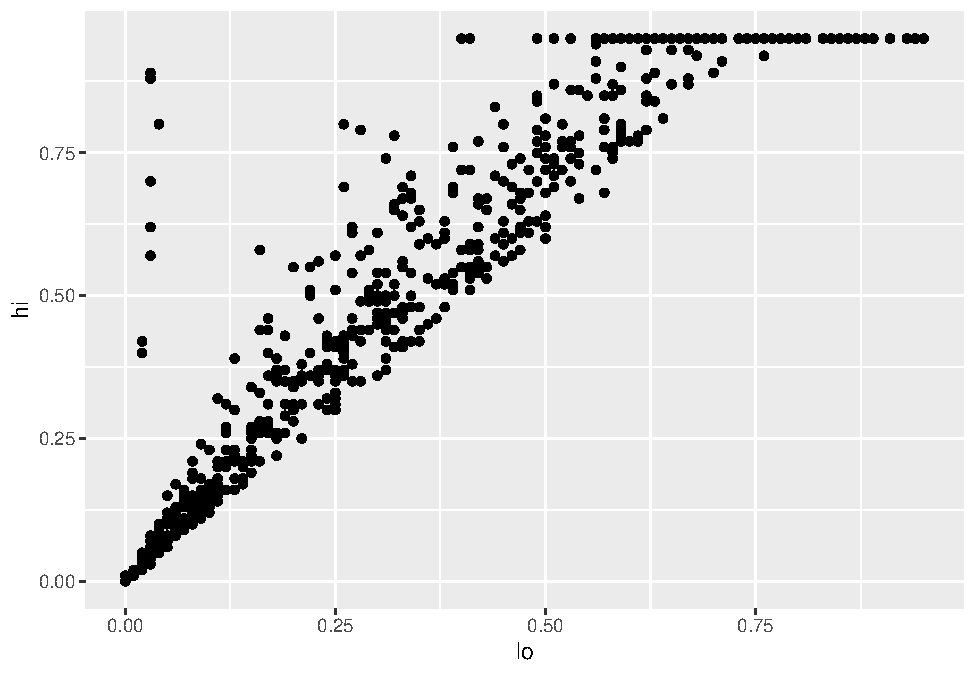
\includegraphics[width=0.8\textwidth]{figures/tidyverse/basic-plot-1.pdf}
  \caption{caption goes here}
  \label{fig:basic-plot-1}
\end{figure}

Looking more closely:

\begin{itemize}
\item
  The function \texttt{ggplot} creates an object to represent the chart with \texttt{infant\_hiv} as the underlying data.
\item
  \texttt{geom\_point} specifies the geometry we want (points).
\item
  Its \texttt{mapping} argument is assigned an \gref{g:aesthetic}{aesthetic},
  which tells \texttt{ggplot} how values are related to the visual aspects of the plot.
  In this case,
  we are telling it that \texttt{lo} is to be used as the $X$ coordinate
  and \texttt{hi} as the $Y$ coordinate.
\item
  The elements of the chart are combined with \texttt{+} rather than \texttt{\pipe} for historical reasons
  (and to prevent us from accidentally include a \texttt{group\_by} in the middle of a plot).
\end{itemize}

Let's create a slightly more appealing plot by dropping NAs,
making the points semi-transparent,
and colorizing them according to the value of \texttt{estimate} (Figure~\ref{fig:plot-after-drop}):

\begin{lstlisting}
infant_hiv %>%
  drop_na() %>%
  ggplot(mapping = aes(x = lo, y = hi, color = estimate)) +
  geom_point(alpha = 0.5) +
  xlim(0.0, 1.0) + ylim(0.0, 1.0)
\end{lstlisting}

\begin{figure}[h]
  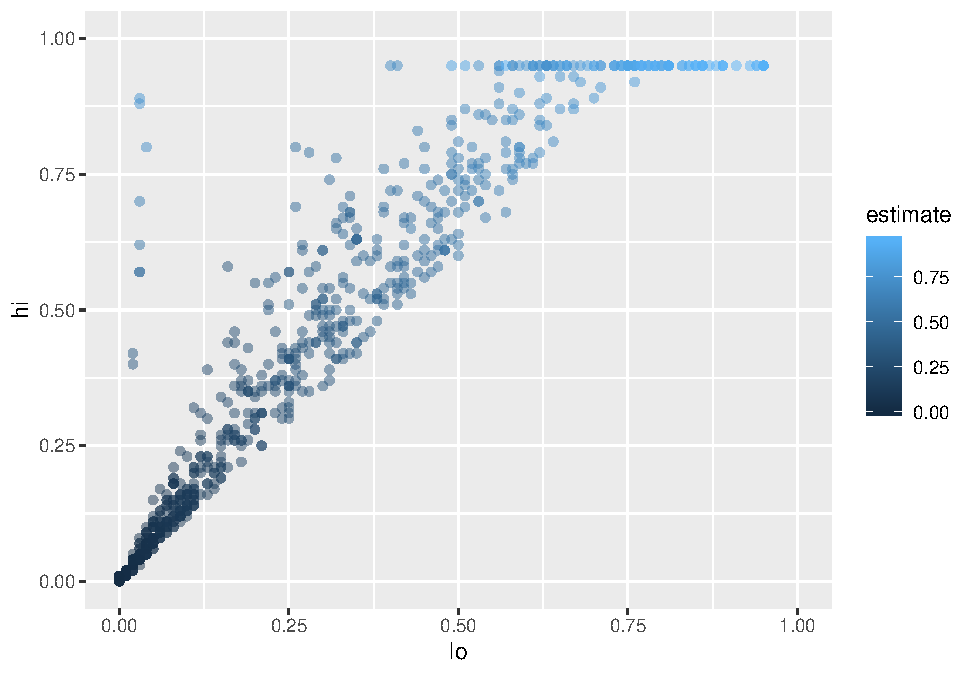
\includegraphics[width=0.8\textwidth]{figures/tidyverse/plot-after-drop-1.pdf}
  \caption{Plot After Dropping NAs}
  \label{fig:plot-after-drop}
\end{figure}

We set the transparency \texttt{alpha} outside the aesthetic because its value is constant for all points;
if we set it inside \texttt{aes(...)},
we would be saying that we want the transparency to vary according to some column in the data.
We specify the limits to the axes manually with \texttt{xlim} and \texttt{ylim} to ensure that the plot includes the upper bounds:
without this,
all of the data would be shown but the upper label ``1.00'' would be omitted.

Figure~\ref{fig:plot-after-drop} shows us that we have some outliers:
there are far more values with \texttt{hi} equal to 0.95 than it seems there ought to be,
and there are eight points running up the left margin that seem troubling as well.
Let's create a new tibble that doesn't have these (Figure~\ref{fig:plot-remove-outliers}):

\begin{lstlisting}
infant_hiv %>%
  drop_na() %>%
  filter(hi != 0.95) %>%
  filter(!((lo < 0.10) & (hi > 0.25))) %>%
  ggplot(mapping = aes(x = lo, y = hi, color = estimate)) +
  geom_point(alpha = 0.5) +
  xlim(0.0, 1.0) + ylim(0.0, 1.0)
\end{lstlisting}

\begin{figure}[h]
  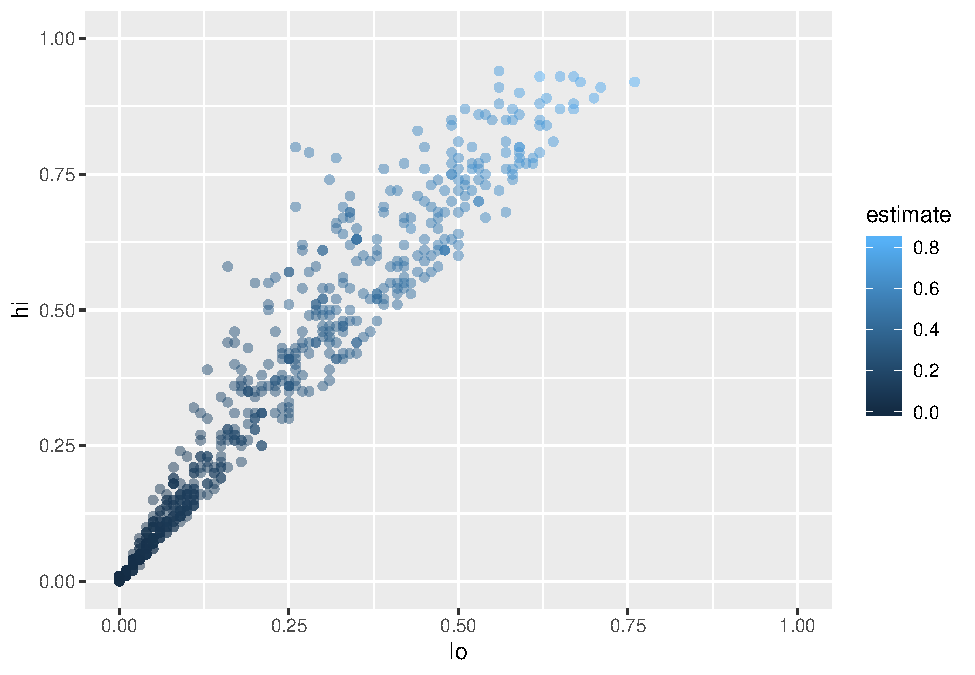
\includegraphics[width=0.8\textwidth]{figures/tidyverse/plot-remove-outliers-1.pdf}
  \caption{Plot After Removing Outliers}
  \label{fig:plot-remove-outliers}
\end{figure}

We can add a fitted curve by including another geometry called \texttt{geom\_smooth}
(Figure~\ref{fig:plot-with-fit}):

\begin{lstlisting}
infant_hiv %>%
  drop_na() %>%
  filter(hi != 0.95) %>%
  filter(!((lo < 0.10) & (hi > 0.25))) %>%
  ggplot(mapping = aes(x = lo, y = hi)) +
  geom_point(mapping = aes(color = estimate), alpha = 0.5) +
  geom_smooth(method = lm, color = 'red') +
  xlim(0.0, 1.0) + ylim(0.0, 1.0)
\end{lstlisting}

\begin{lstlisting}
Warning: Removed 8 rows containing missing values (geom_smooth).
\end{lstlisting}

\begin{figure}[h]
  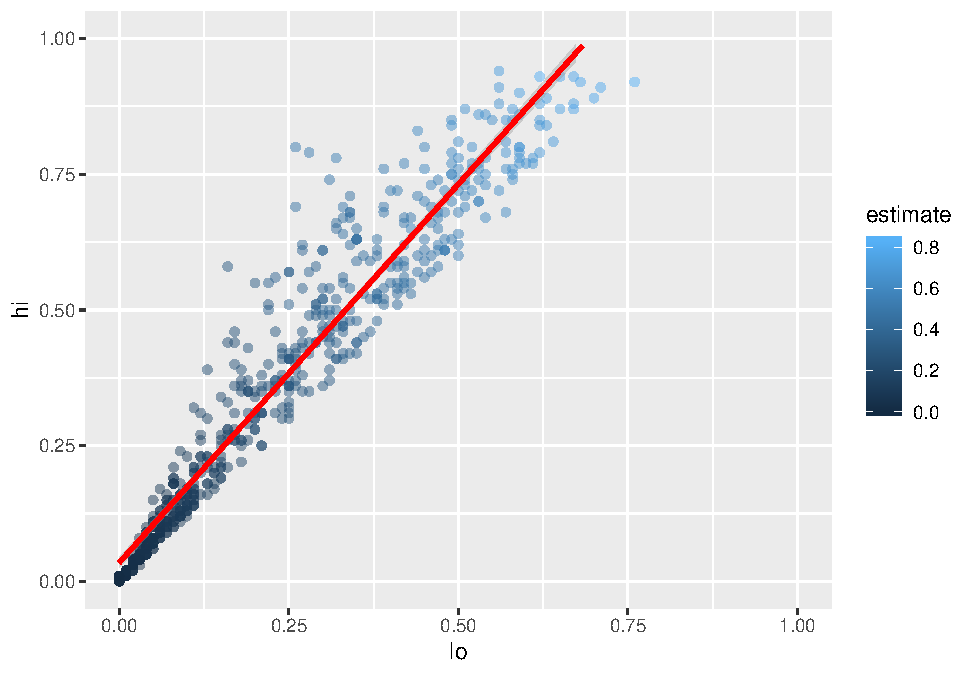
\includegraphics[width=0.8\textwidth]{figures/tidyverse/plot-with-fit-1.pdf}
  \caption{Plot With Fitted Curve}
  \label{fig:plot-with-fit}
\end{figure}

But wait:
why is this complaining about missing values?
Some online searches lead to the discovery that
\texttt{geom\_smooth} adds virtual points above and below the actual data to simplify smoothing calculations,
and that setting \texttt{xlim} and \texttt{ylim} then truncates these\footnote{Remember: differently sane{\ldots}}.
The safe way to control the range of the data is to call \texttt{coord\_cartesian},
which zooms in on a region of interest (Figure~\ref{fig:plot-cartesian}):

\begin{lstlisting}
infant_hiv %>%
  drop_na() %>%
  filter(hi != 0.95) %>%
  filter(!((lo < 0.10) & (hi > 0.25))) %>%
  ggplot(mapping = aes(x = lo, y = hi)) +
  geom_point(mapping = aes(color = estimate), alpha = 0.5) +
  geom_smooth(method = lm, color = 'red') +
  coord_cartesian(xlim = c(0.0, 1.0), ylim = c(0.0, 1.0))
\end{lstlisting}

\begin{figure}[h]
  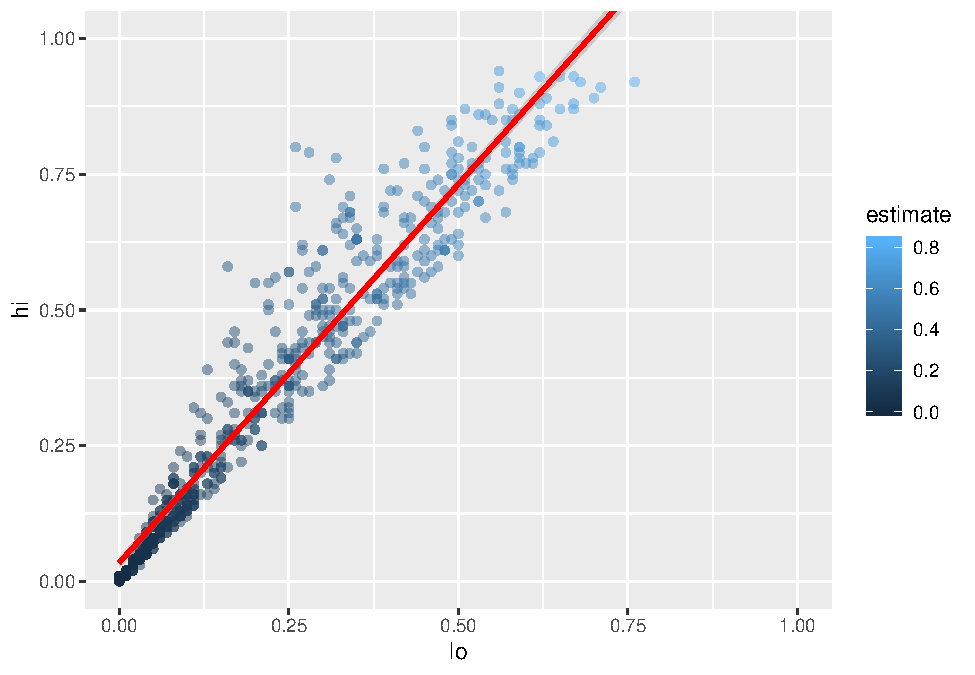
\includegraphics[width=0.8\textwidth]{figures/tidyverse/plot-cartesian-1.pdf}
  \caption{Plot Including Origin}
  \label{fig:plot-cartesian}
\end{figure}

\section{Where can we get more practice using the tidyverse?}

The full text of~\cite{Wick2017} is available online at \url{https://r4ds.had.co.nz/},
and Jeffrey Arnold has posted solutions to all its exercises at \url{https://jrnold.github.io/r4ds-exercise-solutions/}.

\section{Key Points}

\begin{itemize}
\item
  \texttt{install.packages('name')} installs packages.
\item
  \texttt{library(name)} (without quoting the name) loads a package.
\item
  \texttt{library(tidyverse)} loads the entire collection of tidyverse libraries at once.
\item
  \texttt{read\_csv(filename)} reads CSV files that use the string `NA' to represent missing values.
\item
  \texttt{read\_csv} infers each column's data types based on the first thousand values it reads.
\item
  A tibble is the tidyverse's version of a data frame, which represents tabular data.
\item
  \texttt{head(tibble)} and \texttt{tail(tibble)} inspect the first and last few rows of a tibble.
\item
  \texttt{summary(tibble)} displays a summary of a tibble's structure and values.
\item
  \texttt{tibble\$column} selects a column from a tibble, returning a vector as a result.
\item
  \texttt{tibble['column']} selects a column from a tibble, returning a tibble as a result.
\item
  \texttt{tibble[,c]} selects column \texttt{c} from a tibble, returning a tibble as a result.
\item
  \texttt{tibble[r,]} selects row \texttt{r} from a tibble, returning a tibble as a result.
\item
  Use ranges and logical vectors as indices to select multiple rows/columns or specific rows/columns from a tibble.
\item
  \texttt{tibble[[c]]} selects column \texttt{c} from a tibble, returning a vector as a result.
\item
  \texttt{min(...)}, \texttt{mean(...)}, \texttt{max(...)}, and \texttt{std(...)} calculates the minimum, mean, maximum, and standard deviation of data.
\item
  These aggregate functions include \texttt{NA}s in their calculations, and so will produce \texttt{NA} if the input data contains any.
\item
  Use \texttt{func(data, na.rm = TRUE)} to remove \texttt{NA}s from data before calculations are done (but make sure this is statistically justified).
\item
  \texttt{filter(tibble, condition)} selects rows from a tibble that pass a logical test on their values.
\item
  \texttt{arrange(tibble, column)} or \texttt{arrange(desc(column))} arrange rows according to values in a column (the latter in descending order).
\item
  \texttt{select(tibble, column, column, ...)} selects columns from a tibble.
\item
  \texttt{select(tibble, -column)} selects \emph{out} a column from a tibble.
\item
  \texttt{mutate(tibble, name = expression, name = expression, ...)} adds new columns to a tibble using values from existing columns.
\item
  \texttt{group\_by(tibble, column, column, ...)} groups rows that have the same values in the specified columns.
\item
  \texttt{summarize(tibble, name = expression, name = expression)} aggregates tibble values (by groups if the rows have been grouped).
\item
  \texttt{tibble {\pipe} function(arguments)} performs the same operation as \texttt{function(tibble, arguments)}.
\item
  Use \texttt{\pipe} to create pipelines in which the left side of each \texttt{\pipe} becomes the first argument of the next stage.
\end{itemize}

\section{Exercises}

Download \url{FIXME-book-exercises},
unzip this file,
and go into the \texttt{tidyverse} directory to do this chapter's exercises.

\subsection*{People}

\begin{enumerate}

\item
  Load the \texttt{tidyverse} and \texttt{here} libraries.

\item
  Use \texttt{here::here} to construct a path to the file \texttt{person.csv}
  and \texttt{readr::read\_csv} to read that file to create a tibble called \texttt{person}.
  (You can type \texttt{?here::here} to get help on that function,
  or on any other in R.)
  The result should look like this:

\begin{lstlisting}
# A tibble: 5 x 3
  person_id personal_name family_name
  <chr>     <chr>         <chr>      
1 dyer      William       Dyer       
2 pb        Frank         Pabodie    
3 lake      Anderson      Lake       
4 roe       Valentina     Roerich    
5 danforth  Frank         Danforth   
\end{lstlisting}

\item
  Use \texttt{nrow} and \texttt{ncol} to find out
  how many rows and columns the tibble \texttt{person} contains.
  (These names don't have a package prefix because they are built in.)

\item
  Use the pipe operator \texttt{\pipe} and\texttt{dplyr::select}
  (or just \texttt{select}, since we've loaded \texttt{dplyr} as part of the tidyverse)
  to select just the family and personal names from \texttt{person}.
  The result should look like:

\begin{lstlisting}
# A tibble: 5 x 2
  family_name personal_name
  <chr>       <chr>        
1 Dyer        William      
2 Pabodie     Frank        
3 Lake        Anderson     
4 Roerich     Valentina    
5 Danforth    Frank        
\end{lstlisting}

\item
  Use the pipe operator \texttt{\pipe} to add a call to \texttt{filter}
  to the code above
  to produce a table that contains only those people whose family names come in the first half of the alphabet.
  (As in most languages, R lets you compare strings directly using expression like \texttt{name {\textless} 'N'}.)
  The output should look like this:

\begin{lstlisting}
# A tibble: 3 x 2
  family_name personal_name
  <chr>       <chr>        
1 Dyer        William      
2 Lake        Anderson     
3 Danforth    Frank        
\end{lstlisting}

\item
  Use \texttt{mutate} to create a tibble that contains all the columns of \texttt{person}
  plus a new column holding the lengths of everyone's family name.
  The result should look like this:

\begin{lstlisting}
# A tibble: 5 x 4
  person_id personal_name family_name name_length
  <chr>     <chr>         <chr>             <int>
1 dyer      William       Dyer                  4
2 pb        Frank         Pabodie               7
3 lake      Anderson      Lake                  4
4 roe       Valentina     Roerich               7
5 danforth  Frank         Danforth              8
\end{lstlisting}

\item
  Add another stage to the pipeline to sort rows in descending order by length to create this table:

\begin{lstlisting}
# A tibble: 5 x 4
  person_id personal_name family_name name_length
  <chr>     <chr>         <chr>             <int>
1 danforth  Frank         Danforth              8
2 pb        Frank         Pabodie               7
3 roe       Valentina     Roerich               7
4 dyer      William       Dyer                  4
5 lake      Anderson      Lake                  4
\end{lstlisting}

\end{enumerate}

\subsection*{Measurements}

\begin{enumerate}

\item
  Read the file \texttt{measurements.csv} to create a new tibble called \texttt{measurements}
  that looks like this:

\begin{lstlisting}
# A tibble: 21 x 4
   visit_id person_id quantity reading
      <dbl> <chr>     <chr>      <dbl>
 1      619 dyer      rad         9.82
 2      619 dyer      sal         0.13
 3      622 dyer      rad         7.8 
 4      622 dyer      sal         0.09
 5      734 pb        rad         8.41
 6      734 lake      sal         0.05
 7      734 pb        temp      -21.5 
 8      735 pb        rad         7.22
 9      735 <NA>      sal         0.06
10      735 <NA>      temp      -26   
# ... with 11 more rows
\end{lstlisting}

\item
  Use the functions \texttt{filter} and \texttt{is.na}
  to create a new table called \texttt{cleaned}
  that contains only the records that \emph{aren't} missing a value for the \texttt{reading} column.

\item
  Use \texttt{group\_by} and \texttt{summarize}
  to group the values in \texttt{cleaned} by the quantity measured
  (salinity, temperature, or radiation)
  and count the number of measurements of each kind.
  The result should look like this:

\begin{lstlisting}
# A tibble: 3 x 2
# Groups:   quantity [3]
  quantity     n
  <chr>    <int>
1 rad          8
2 sal          7
3 temp         3
\end{lstlisting}

\item
  Use \texttt{group\_by} and \texttt{summarize}
  to count the number of measurements of each of the three kinds.
  The result should be:

\begin{lstlisting}
# A tibble: 3 x 4
  quantity    low    mid  high
  <chr>     <dbl>  <dbl> <dbl>
1 rad        1.46   6.56  11.2
2 sal        0.05   9.24  41.6
3 temp     -21.5  -18.7  -16  
\end{lstlisting}

\item
  Most of the salinity measurements lie between 0 and 1,
  but a handful range up to 100.
  During a brief interval of lucidity,
  the librarian who collected the battered notebooks from which the data was transcribed
  informs us that one of the explorers recorded percentages rather than actual values.
  Look up the documentation for the function \texttt{ifelse}
  and then use it to divide all salinity values greater than 1.0 by 100.
  The result should look like this:

\begin{lstlisting}
# A tibble: 18 x 4
   visit_id person_id quantity reading
      <dbl> <chr>     <chr>      <dbl>
 1      619 dyer      rad        9.82 
 2      619 dyer      sal        0.13 
 3      622 dyer      rad        7.8  
 4      622 dyer      sal        0.09 
 5      734 pb        rad        8.41 
 6      734 lake      sal        0.05 
 7      734 pb        temp     -21.5  
 8      735 pb        rad        7.22 
 9      751 pb        rad        4.35 
10      751 pb        temp     -18.5  
11      752 lake      rad        2.19 
12      752 lake      sal        0.09 
13      752 lake      temp     -16    
14      752 roe       sal        0.416
15      837 lake      rad        1.46 
16      837 lake      sal        0.21 
17      837 roe       sal        0.225
18      844 roe       rad       11.2  
\end{lstlisting}

\end{enumerate}

\subsection*{Home Range Areas}

\begin{enumerate}

\item
  The file \texttt{home-range-database.csv} contains data
  on the home range areas (HRAs) of various species~\cite{Tamb2015}.
  Read in this data and store the values in a tibble called \texttt{hra}.

\item
  Fill in the code below to create a histogram of the values in \texttt{mean.mass.g}
  (mean mass in grams).
  The result should look like Figure~\ref{fig:chart-mass-1}.
  
\begin{lstlisting}
ggplot(hra) +
  geom_histogram(mapping = ____)
\end{lstlisting}

\begin{figure}[h]
  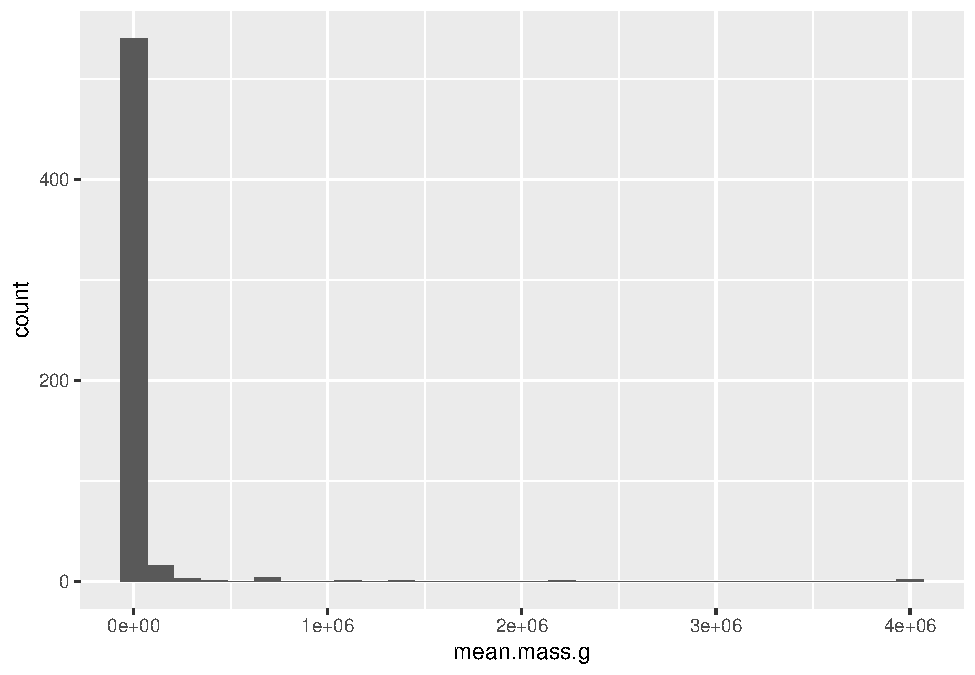
\includegraphics{figures/practice/chart-mass-1.pdf}
  \caption{Animal Masses}
  \label{fig:chart-mass-1}
\end{figure}

\item
  Create a new histogram showing the logarithms of the masses
  (which are helpfully precalculated in \texttt{log10.mass}).
  Add titles and labels so that the result look like Figure~\ref{fig:change-visual-1}.

\begin{figure}[h]
  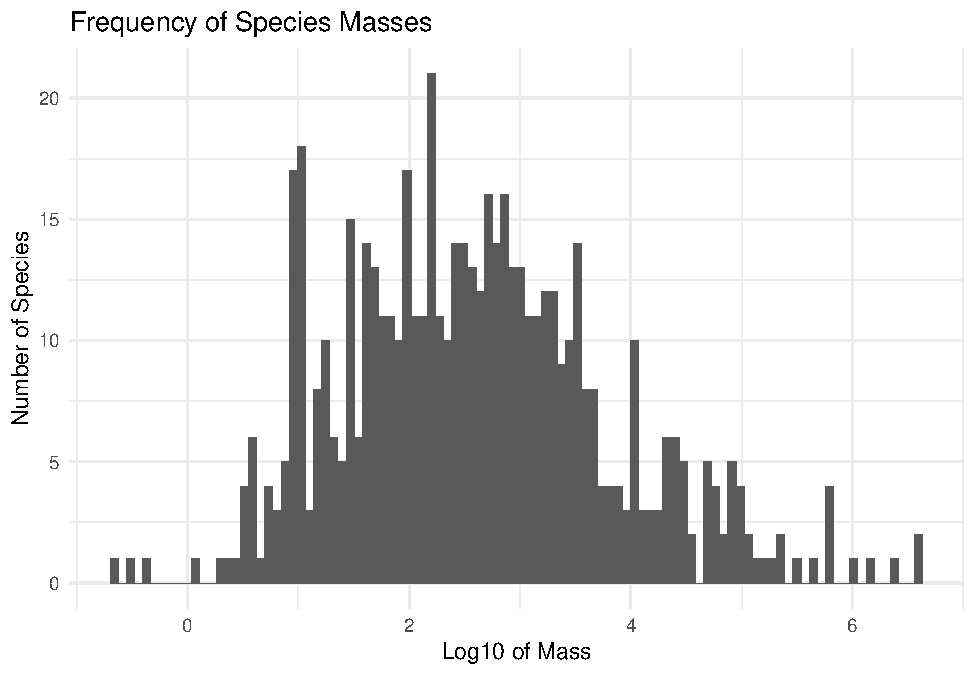
\includegraphics{figures/practice/change-visual-1.pdf}
  \caption{A Tidier Version}
  \label{fig:change-visual-1}
\end{figure}

\item
  Use \texttt{geom\_point} to create a scatter plot showing
  the relationship between \texttt{log10.mass} and \texttt{log10.hra}.
  The result should look like Figure~\ref{fig:scatterplot-1}.

\begin{figure}[h]
  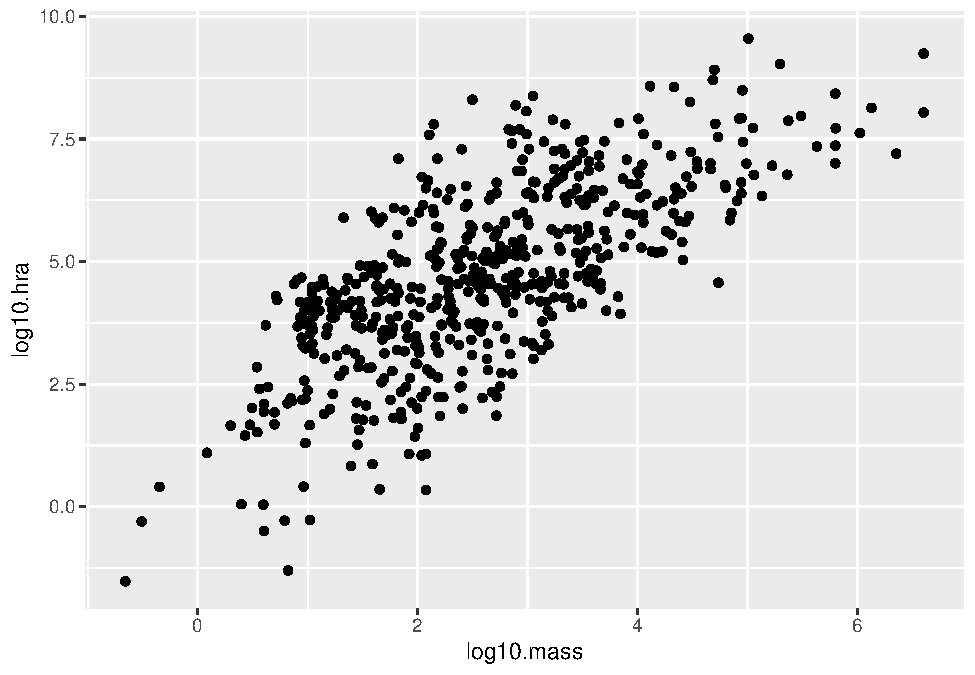
\includegraphics{figures/practice/scatterplot-1.pdf}
  \caption{Mass vs.\ Home Range Area}
  \label{fig:scatterplot-1}
\end{figure}

\item
  Explain how each line in the code below helps create the plot in Figure~\ref{fig:fit-line-1}.

\begin{lstlisting}
hra %>%
  filter(class == "aves") %>%
  ggplot(mapping = aes(x = log10.mass, y = log10.hra)) +
  geom_point(alpha = 0.5) +
  geom_smooth(method = lm, color = 'red')
\end{lstlisting}

\begin{figure}[h]
  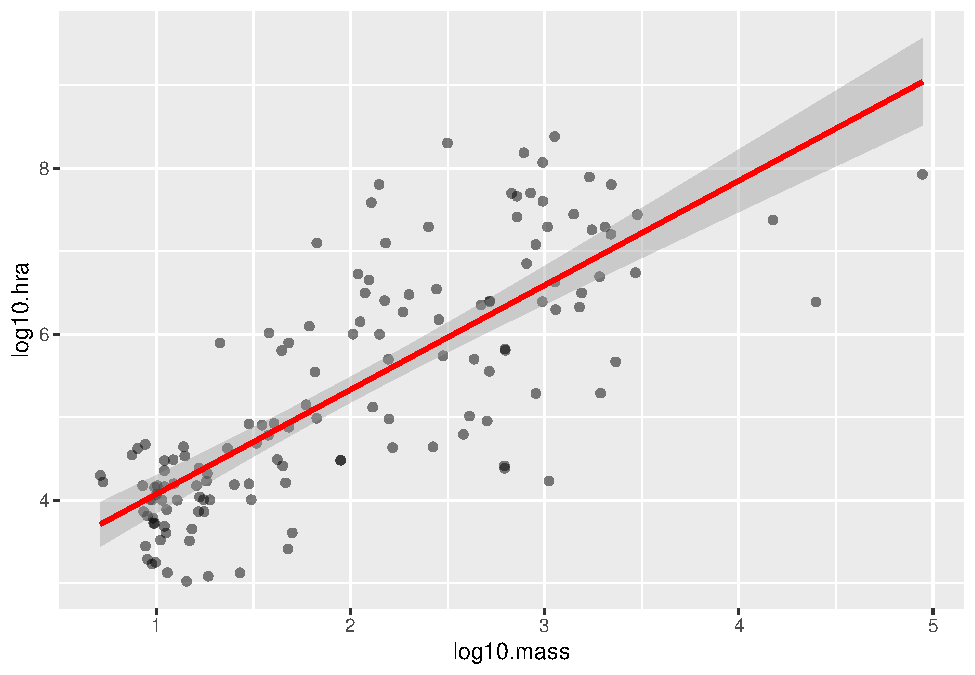
\includegraphics{figures/practice/fit-line-1.pdf}
  \caption{Fitting a Regression Line}
  \label{fig:fit-line-1}
\end{figure}

\end{enumerate}
